\subsection{传输对象模式}

传输对象模式用于从客户端向服务器一次性传递带有多个属性的数据。在这里我们设计了TraceLogTO类作为要传输的业务对象,其内部包含了TraceLogMO类的数据。设计TraceLogBO类作为业务对象类,用于向客户端(即MVP模式中的TraceLogModel类)传输数据,以及从客户端获取新添加的traceLog信息。

\begin{figure}[htb]
  \centering
  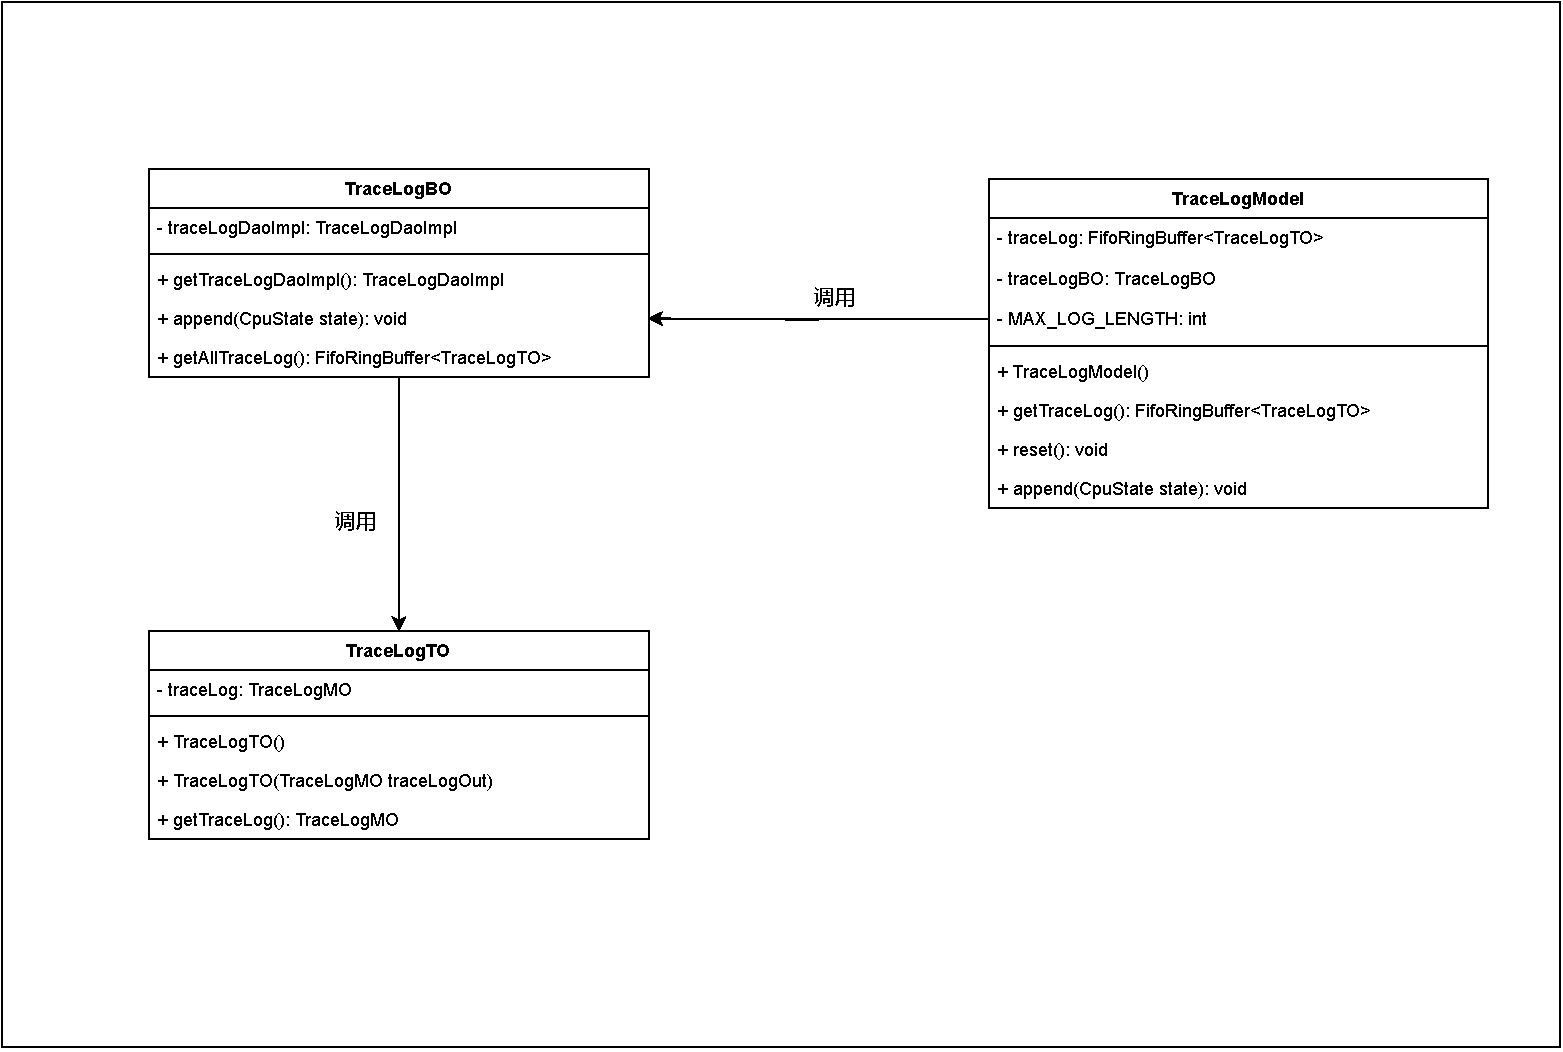
\includegraphics[width=0.9\textwidth]{figures/传输对象模式.pdf}
  \caption{传输对象模式在 Slow6502 中的类图}
\end{figure}
